\section{Demonstration of the rate of convergence in Matlab}\label{sec:matlab}
In this section, we analyse the rate of convergence by comparing the plots of error norms against the number of iterations.

In section \ref{sec:dichotomy results}, we have proved the \emph{Von-Neumann Halperin Dichotomy} which states that:

If $M_i$  ($1\leq i\leq r$ ) are closed subspaces in the Hilbert space $X$, and $M:=\bigcap_{i}^r M_i$, then for $T=P_{r}P_{r-1}\cdots P_{1}$ where $P_{i}$ is the orthogonal projection on $M_i$, exactly one of the two following statements holds:
\begin{enumerate}
\item $\sum_{i=1}^r M_{i}^{\perp}$ is closed, then there exists $\alpha\in [0,1)$ and $c\in \mathbb{R}$ such that $\|T^n-P_{M}\|\leq c\alpha^n$ for each $n$.
\item $\sum_{i=1}^r M_{i}^{\perp}$ is not closed, then for each $(r_n)\in c_0$, $r_n\in\mathbb{R}^{+}$, for all $x\in X$, $\|T^n x-P_{M}x\|\neq O(r_n)$.
\end{enumerate}

In fact, we can replace (b) by arbitrarily slow convergence, that is,
for each $(r_n)\in c_0$, $r_n\in\mathbb{R}^{+}$, there exists $x\in X$ such that $\|T^n x-P_{M}x\|\geq r_n$ for each $n\in\mathbb{N}$\cite{DH10a}. 

In \emph{Deusch} and \emph{Hundal's} recent work\cite{DH15}, they suggest  that the $x\in X$ satisfies $\|T^n x-P_{M}x\|\geq r_n$ for all $n$ must be chosen from $X\setminus(M\oplus(M_1^{\perp}+M_2^{\perp}))$.

In the application of Schwarz Altenrating Method for the Neumann problem in the two-dimensional domain, we have showed that $M=\{0\}$, so the $x$ have to be chosen from $H^1(\Omega)\setminus (M_1^{\perp}+M_2^{\perp})$.

In order to test the above conjecture, we claim that for $u\in C(\overline{\Omega})\cap(M_1^{\perp}+M_2^{\perp})$, we have $u(x)=0$ for all problematic points on $\partial\Omega$.  The claim is indeed true due to the following fact: if $u\in C(\overline{\Omega})\cap H^1(\Omega)$, then there exists $\phi_n\in C^{\infty}(\overline{\Omega})$ such that $\|u-\phi_n\|_\infty\rightarrow 0$ as $n\rightarrow \infty$.

Since $u\in C(\overline{\Omega})\cap(M_1^{\perp}+M_2^{\perp})=C(\overline{\Omega})\cap (Y_1+Y_2)=C(\overline{\Omega})\cap Y=C(\overline{\Omega})\cap \overline{Z}$ where $$Z=\{u\in C^{\infty}, u=0 \mbox{ near the problematic points}\},$$ there exists $u_n\in C^{\infty}(\overline{\Omega})\cap Z$ such that $\|u-u_n\|_{\infty}\rightarrow 0$ as $n\rightarrow \infty$.  $u_n=0$ on problematic points implies that $u(x)=\lim_{n\rightarrow} u_n(x)=0$ for all problematic points on $\partial \Omega$. 

Thus for $x_0\in H^1(\Omega)\setminus (M_1^{\perp}+M_2^{\perp})$, we need $x_0\neq 0$ at problematic points, that is, $u_0\neq u$ at problematic points for $u, u_0\in H^1(\Omega)$.


Consider the neumann problem 
$$\begin{cases}
-\Delta u+u=1, \\
\frac{\partial u}{\partial r}=0\\
\end{cases}$$
on a L-shape domain as shown in Figure 4.1.
\begin{figure}[t]
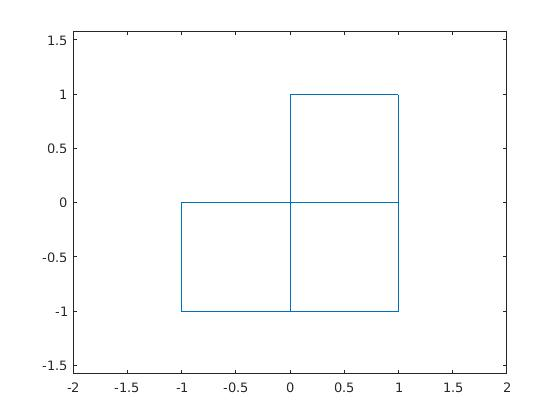
\includegraphics[width=\textwidth]{lshape.jpg} 
\caption{lshape domain}
\end{figure}

It is easy to see that the true solution is $u\equiv 1$. 

If we set $u_0=|\log(\frac{1}{\sqrt{(x^2+y^2)}})|^\alpha$ for $\alpha\in (0,0.5)$, $u_0=\infty$ at the problematic point $(0,0)$, then the surface plot of the solution after $80$ iterations is shown in Figure 4.2. (Details of the Matlab code can be found in Appendix \ref{sec:appA})

\begin{figure}[h]
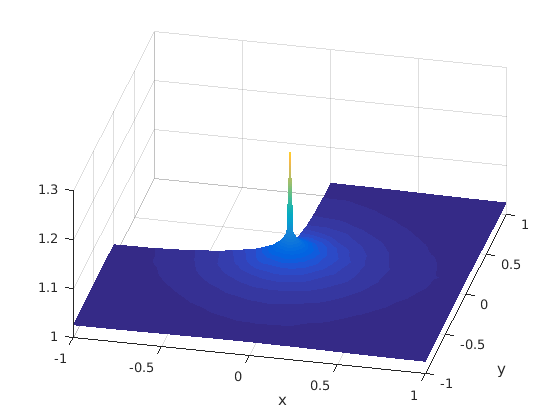
\includegraphics[width=\textwidth]{verybadinitial_u.png}
\caption{surface plot of the solution $u_n$}
\end{figure}

We plot both $\log(\|u_n-u\|_\infty)$ and $\log(\|u_n-u\|_{H1})$ against the number of iterations with respect to different mesh sizes to demontrate the rate of convergence.

\begin{figure}[h]
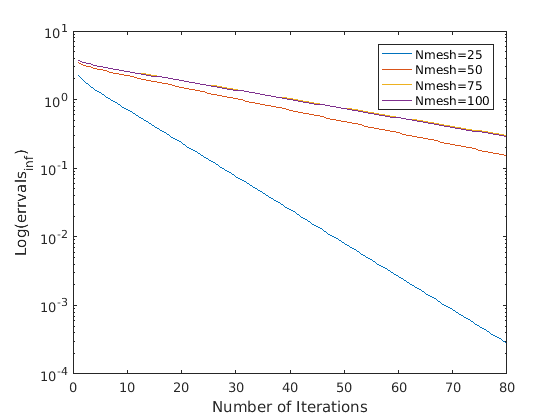
\includegraphics[width=\textwidth]{verybadinitial_infnorm.png}
\caption{The plots of $\log(\|u_n-u\|_\infty)$ against number of iterations}
\end{figure}
\begin{figure}[h]
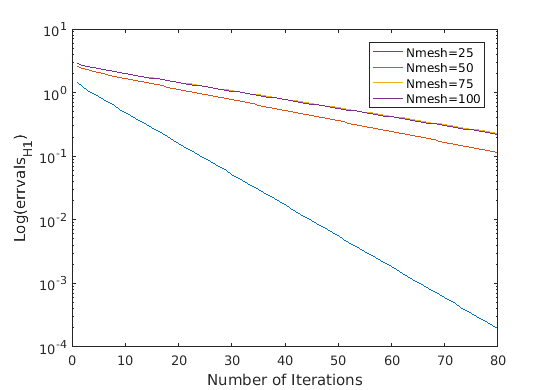
\includegraphics[width=\textwidth]{verybadintial_H1norm.png}
\caption{The plots of $\log(\|u_n-u\|_{H1})$ against number of iterations }
\end{figure}

As we can observe from Figure 4.3 and Figure 4.4, the rate of convergence decays as the number of iterations increase with respect to both the infinity and $H_1$ norms. The results shown on the two error plots are compatible with \emph{Deutsch} and \emph{Hundal's} conjecture.

From the plots we can also deduce that the rate of convergence decreses when we refine the mesh near the problematic point. After we refine the mesh to a certain scale (i.e.Nmesh$=75$ in our plot), the plot will no longer depend on the mesh size.

\begin{figure}[h]
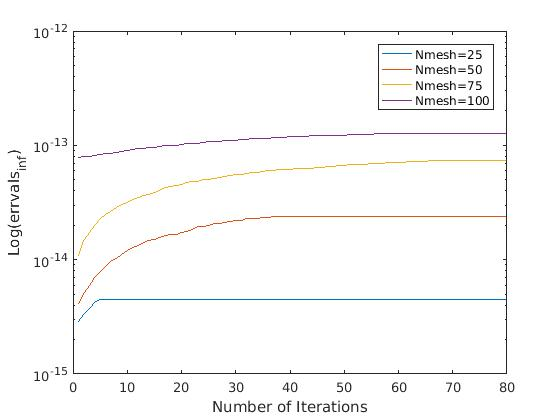
\includegraphics[width=\textwidth]{goodinitial_inf.jpg}
\caption{The plots of $\log(\|u_n-u\|_{\infty})$ against number of iterations }
\end{figure}

Now we start with a good initial guess, $u_0=1-\sin(22x)sin(10y)$, which gives $u_0=1$ on the problematic point. Again, we plot the two error norms against the number of iterations.
\begin{figure}[h]
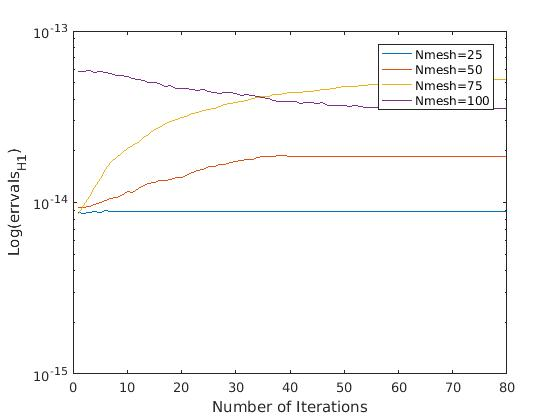
\includegraphics[width=\textwidth]{goodinitial_H1.jpg}
\caption{The plots of $\log(\|u_n-u\|_{H1})$ against number of iterations }
\end{figure}
 
From \emph{Deutsch} and \emph{Hundal's} conjecture, we expect exponentially fast convergence, that is, straight lines for the plots of both $\log(\|u-u_n\|_{\infty})$ and $\log(\|u-u_n\|_{H1})$ against the number of iterations.
However, the plots shown on Figure 4.5 and Figure 4.6 are bizarre for the first few iterations. I suspect that this is because the numerical solutions we obtained from solving PDEs on different domains are approximate values only. Since the soluitons are pointwise values, we try to decrease our grid size, that is, to increase the number of plots ( change Nplot$=101$ to Nplot=$2001$) to increase their accuracy.  We plot the first few iterations in Figure 4.7 and Figure 4.8 to see whether there is any improvement. 
\begin{figure}[h]
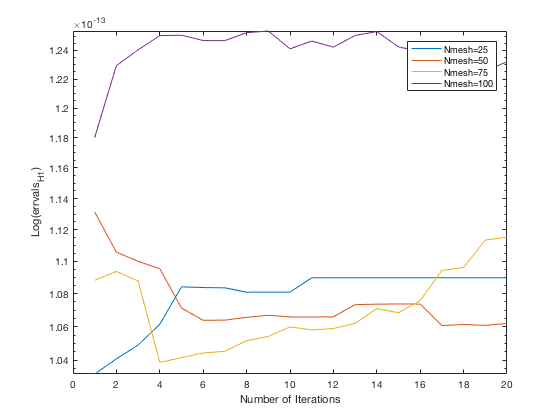
\includegraphics[width=\textwidth]{smallgridsize.png}
\caption{The plots of $\log(\|u_n-u\|_{H1})$ against number of iterations }
\end{figure}
\begin{figure}[h]
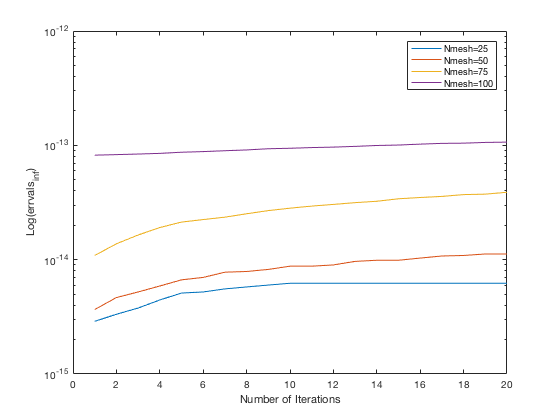
\includegraphics[width=\textwidth]{smallgridsize2.png}
\caption{The plots of $\log(\|u_n-u\|_{\infty})$ against number of iterations }
\end{figure}
\par
Surprisingly, the plots are inconsistent with what we expect as well. In fact, the plots are reasonable in some sense since the errors are quickly within machine precision. 
